%!TEX root = ./BPM17.tex


\section{Background} % (fold)
\label{sec:background}
%%%% CONTENT
% background + related work
In this section, we report the background concepts useful for understanding the remainder of the thesis.



\subsection{Event Logs and Traces} \label{logs}

Most of the huge enterprises and middle sized companies have a lot of processes being executed. With the rapid development of database technology and inexpensiveness of data warehouses saving all the transactional data in the company became a must. Most of this data is about processes that are happening in the company. Those range from core processes such as "order to cash" and "issue to resolution" to additional such as managerial processes. The nature of this information is processlike (sequential) so they are usually being recorded in the format of logs. 

An event log is a set of traces, each representing the execution of a process (case instance). Each trace consists of a sequence of activities, each referring to the execution of an activity in a finite activity set $A$.

\begin{definition}[Trace, Event Log]
	A trace $\sigma=\left\langle a_1, a_2, ... a_n\right\rangle \in A^*$ over $A$ is a sequence of activities. An event log $L \in \cal{B}$(A) is a multi-set of traces over the activity set $A$.
\end{definition}

A \emph{prefix of length} $k$ of a trace $\sigma=\left\langle a_1, a_2, ... a_n\right\rangle \in A^*$, is a trace $p_k(\sigma)=\left\langle a_1, a_2, ... a_k\right\rangle \in A^*$ where $k \leq n$; the \emph{suffix of the prefix of length} $k$ is defined as the remaining part of $\sigma$, that is, $s_k(\sigma) = \left\langle a_k+1, a_k+2, ... a_n\right\rangle \in A^*$. For example, the prefix of length $3$ of $\npla{a,c,r,f,s,p}$ is $\npla{a,c,r}$, while the suffix of this prefix is $\npla{f,s,p}$.

A \emph{cycle} in a trace $\sigma \in A^*$ is a sequence of activities repeated at least twice in $\sigma$ (with adjacent repetitions). For example, trace $\npla{a,b,a,b,a,b,c,d,e,f,g,e,f,g,c,d}$ contains two cycles: $\npla{a,b}$ (3 repetitions) and $\npla{e,f,g}$ (2 repetitions).

Speaking practically, the log is a set of process executions (Traces). Trace is a set of events happened in the sequence.

Sequence is defined by timestamps. They are the first essential part of the process. Every correctly stored process must contain the time stamps of when certain activity was performed. 

Trace should have an identification, that is the case ID. Whenever the real world process starts the new case ID is created. That to ensure granularity of the data values. In the issue to resolution process the ID refers to unique number associated with one instance of the issue raised. 

The third essential element of a trace is an Activity ID. These are the names of different activities performed during one instance of the process. For our example these might be "issue recorded", "decision made", "solved", "confirmation received", or "issue canceled". These provide an understanding of what the process is actually performing. 

Many other data values can be recorded. Let's look at the real world exampl in the figure e~\ref{figure:trace-example-1} from the dutch hospital log. The figure shows one event of the process. 

\begin{figure}[!ht]
	\begin{center}  
		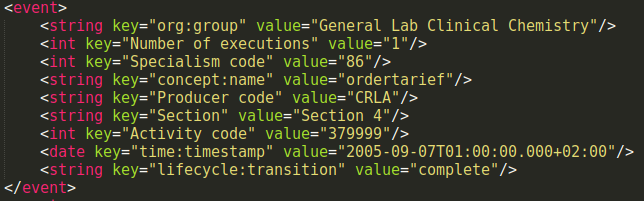
\includegraphics[width=\textwidth]{3_event_example.png}
		\caption{Trace example, exempt from the BPI11 hospital log~\cite{bpichallenge2011}}
		\label{figure:trace-example-1}	
	\end{center}
\end{figure}

One can see that the timestamp is present and one can define case id to be "Activity code" and activity ID as "concept:name".

There are number of other parameters such as "org:group" that shows the department in the clinic, "Number of executions" that shows number of times certain operation was performed and others.  All parameters combined give the best picture of the process execution, therefore it is important for methods exploiting logs to use most complete data set possible.

Furthermore, the logs can contain text information such as comments or emails, bringing up the complexity level of the problem. Text mining methods in conjunction with sequence classification should be used to bring down the problem~\cite{DBLP:conf/bpm/TeinemaaDMF16}.

As for example in the hospital log mentioned above, it might be a parameter with comments from the doctor for patient wellbeing. 

In the data based systems, the log can be stored in different structures. Enterprise Resource Planning (such as SAP, Oracle) systems have their own data format of journaling the data. It can also be CSV spreadsheet (figure~\ref{figure:trace-example-2_csv}) or XES formatted log (shown in figure ~\ref{figure:trace-example-1}).  

\begin{figure}[!ht]
	\begin{center}  
		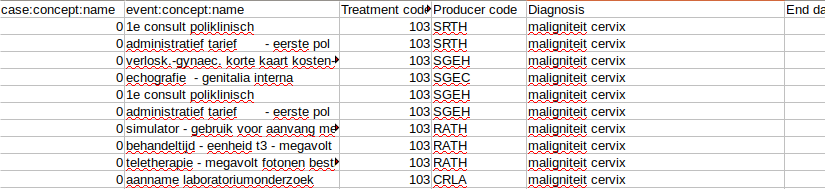
\includegraphics[width=\textwidth]{4_event_example_csv.png}
		\caption{Trace example (CSV format), exempt from the BPI11 hospital log~\cite{bpichallenge2011}}
		\label{figure:trace-example-2_csv}	
	\end{center}
\end{figure}



\subsection{Process mining}

\todo{More of this! }

Process mining is a business process management technique that enables the analysis of processes based on the event logs. The main idea is improving business processes based on analysis of the logs as sequential and continuous processes. This is what makes it different from the methods established in data mining and business intelligence which treat the data as set of distinct events to gather insights. 

As a rule the methods of process mining applied mostly to the processes that do not have formal description or have consistent deviations from the ones predicted in the system. 

The three main activities performed under the process mining field are:

\begin{itemize}
	\item \textbf{Process analysis (Discovery):} encompasses all methods to discover insights from the past process executions. As an example would be the issue to resolution process from the insurance company. Process discovery methods allow building abstract representation of an event log. The goal of this is to build approximated model that delivers better insights into the underlined processes. Discovered models can be in forms of BPMN models, Petri nets, and declarative rules. 
	\item \textbf{Conformance analysis:} it takes existent formalized models and check them against real log. In detail, that means that the business process analyst has the BPMN model for the process created (or generated). And now, the goal is to match the real processes to the model (mostly interest is in doing it on a fly). That is done in order to check for any deviations the process can have, and if possible to for prevention on undesired behavior.
	\item \textbf{Process enhancement:} it helps to use logs in order to enhance current executions of the processes. The information of the past is used to change the model and how the processes are being performed.
\end{itemize}
 


\subsection{Predictive monitoring}

Predictive monitoring is an advancing subfield of Process Mining. As a subfield of Process Mining, its main focus also lies in exploring and exploiting the process logs (the process executions). More specifically, predictive monitoring encompasses the methods that deal with online predictions of process outcomes. The outcome of interest can be compliance of with a measure (for example in an order to cash process the measure can be that any of the financial operations that involve an amount more then 2500 euro, are not performed without confirmation from the top financial officer), achieving objective (such as in issue to resolution process, if the process will be completed under 7 days time), or classifications (giving a label to the uncompleted trace, such as issue resolved, or not).  
\par
Many algorithms are applied to solve above mentioned problems, for example classic machine learning algorithms as classification and clustering~\cite{Leontjeva2015}. More complex concepts are also used, such as Markov models~\cite{Leontjeva2015}, time series~\cite{Lam20096986}, and deep learning~\cite{niek96732,evermann,quteprints96732} approaches. 
\par
In order to successfully apply these algorithms for facing the problems, it is necessary to have solid understanding on the process log nature. The aspects that can come into play, are the data types (while the case ID and activity ID are defined as categorical values, we have to deal with time stamps that are basically real valued, also text comments that are strings, or other numerical values such as sums of money), stationarity (it usually refers to time series data that have a stable mean, variance etc. over time. Best example from process logs are timestamps. One should account that they represent only the moment in an absolute time scale, while algorithms would only work if the input will be a relative measure, such as difference between timestamps). 
\par
Keeping in mind definition of the business process log from the section~\ref{logs} one can easily find the caveats in the early process mining approaches, that tend to ignore the data payload, taking into consideration only the control-flow (sequence of activities). Some of the approaches do the opposite, that is consider data, without control-flow~\cite{vanderAalst2010,DBLP:journals/is/AalstSS11,Schonenberg2008}. In that case the traces are considered to be a simple sequences. Moreover, methods introduced usually designed to work in offline fashion, exploring uncompleted cases. But, to make more accurate, mature, online predictions one should leave out neither payload nor control-flow information. That's when the Complex Symbolic Sequences as methods of encoding of a log are introduced. 


\subsection{Encodings of business logs}

Every machine learning problem needs the data represented in a particular way. To solve problem one needs to be aware that it is always a trade-off between the model used and the way of data encoding. 

In the next subsections the descriptions of the most used encodings are given.


\subsubsection{Simple symbolic sequence encoding}

This encoding is inherited from a massive number of works in machine learning and statistics such as concerning applications in health-informatics~\cite{Xing:2010:BSS:1882471.1882478}, or anomaly detection in Unix access systems, determining fraud users by its query log sequences. 

The simple symbolic sequence could be formalized as follows: $seq_{k} = (a_j)_{j=1}^{n}$.
Where the $seq_{k}$ is one trace in the log.


\begin{figure}[!ht]
	\begin{center}  
		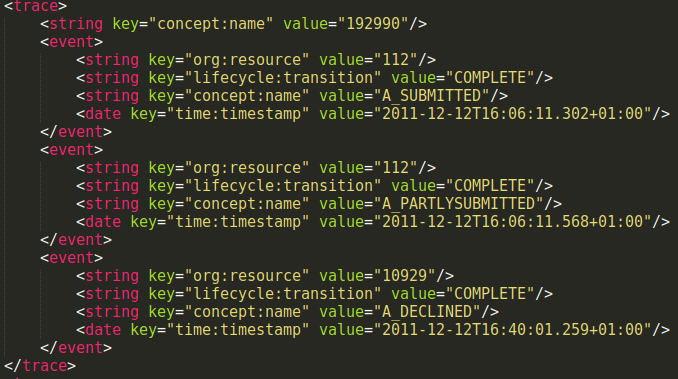
\includegraphics[width=\textwidth]{5_log_example_fin.png}
		\caption{Trace example, exempt from the BPI12 financial log~\cite{bpichallenge2012}}
		\label{figure:trace-example-2}	
	\end{center}
\end{figure}


As an example let's take a financial log from the bpi challenge. On the figure~\ref{figure:trace-example-2} one trace is shown.

So if we formalize this trace to the simple symbolic sequence from this log (considering activity ID to be "concept:name") it will have a form:

$seq = ("A\_SUBMITTED","A\_PARTLYSUBMITTED","A\_DECLINED")$

Simple Symbolic Sequences, however, have limitations that prevent getting best results of their use.

That is because simple symbolic sequences discard most of the rich information present in process logs, that is not limited to control-flow. An example would be the log in the big fast food chain, where the process about their employee's actions is daily recorded into the log. In Table~\ref{tab:statements}, you can see that log of this nature contains static features, control-flow components and number of dynamic features. Static feature include ID of the employee, and his age. Dynamic features are the $t_i$ that is the time spent working, $rID_i$ is an ID of the restaurant that employee worked in on that day, $rev_i$ money he earned for the company. 

\begin{table}[h]
	\centering
	\begin{tabular}{| l | l | l | l | l | l | l | l | l | l | l | l |}
		\hline
		& Age & ID & t\_1 & .. & t\_n & rID\_1 & .. & rID\_n & rev\_1 & .. & rev\_n \\	
		\hline
		tr1 & 20 & 00123 & 28800 & .. & 24840 & 11 & .. & 12 & 120\$ & .. & 112\$ \\
		tr2 & 24 & 00023 & 16890 & .. & 23460 & 12 & .. & 12 & 80\$ & .. & 111\$ \\
		tr3 & 18 & 01129 & 23804 & .. & 17897 & 11 & .. & 11 & 340\$ & .. & 23\$ \\
		tr4 & 21 & 00772 & 40034 & .. & 24564 & 12 & .. & 12 & 130\$ & .. & 2\$ \\
		\hline
	\end{tabular}
	\caption{Example of Complex Symbolic Sequence encoding}
	\label{tab:statements}
\end{table}


As well as the data used in areas described in the beginning on this chapter can be easily represented as simple symbolic sequence, there are many algorithms developed to work with. There are feature based classifications, sequence distance based, support vector machines, or model based classification~\cite{Xing:2010:BSS:1882471.1882478}. That's why first attempts to make predictions of the business processes were made with the use of this simple encodings.


\subsubsection{Complex symbolic encoding} \label{complex-sym-enc}

On contrary to Simple Symbolic Sequence encodings, the Complex Symbolic Sequences are introduced~\cite{Leontjeva2015} and we can capture much more information about log. Complex Symbolic Sequence is basically ordered list of vectors, where each vector is a subset of some alphabet inferred from the log.

When Complex Symbolic Sequences are used instead of Simple Symbolic Sequences for dealing with prediction problems, the complexity space of the prediction problem grows substantially. So it suggests to use new and more complex approaches to work with them.

Some of the base lines of working with complex symbolic sequences use index-based encodings, and index latest payload encodings mentioned in following paper~\cite{Leontjeva2015}.   

To exemplify this approach for encodings lets again take a look at the log in figure~\ref{figure:trace-example-2}. The Complex Symbolic Sequence form of this log will have following representation:

\begin{table}[h]
	\centering
	\begin{tabular}{| l | l | l | l | l | l | l | l | l |}
		\hline
		& $concept:n_{1}$ & .. & $concept:name_{3}$ & $org:resource_{1}$ & .. & $org:resource_{3}$ & $time:timestamp_{1}$ & .. \\	
		\hline
		tr1 & A\_SUBMITTED & .. & A\_DECLINED &  112 & .. & 10929 &  2011-12-12T16:06:11 & ..  \\
		tr2 &  & .. & .. & .. & .. & ..  & .. & ..  \\
		\hline
	\end{tabular}
	\caption{Example of Complex Symbolic Sequence encoding}
	\label{tab:complesymbseq_log_example}
\end{table}


Additionally, Complex Symbolic Sequence encoding can have textual data encoded as additional parameters. For that its needed to use the text knowledge extraction techniques, such as described below.

First step the data is preprocessed. It is done in few steps. Firstly, text is segmented by tokenization. Then, the text is normalized, to eliminate word differences such as "e-mail" and "email". Later, \textit{lemmatization} is used to bring same words of different grammatical form to the single form. Words such as "go" and "went" are grouped with the "go" label.

Next step is encoding. The most used methods~\cite{DBLP:conf/bpm/TeinemaaDMF16}:

\begin{enumerate}
	\item \textit{Bag-of-n-grams} is a method, based on BoNG model. It has two parameters, $n$ - maximum size of $n$-grams, and $idf$ boolean variable specifying if the model is normalized. The $n$-gram means scoring feature representation based on the every sequence of $n$ words. Normalization is used in order not to favor words that are relatively popular in one document.
	
	By the result of this procedure, the vector will be build in the following form:
	
	Having vocabulary:
	\[V(1)=("send","phone","radio","play","it","is","you","like", "say").\]
	And the input sentence "You said you like radio".
	
	The resulting vector will be of the form: 
	
	$d^j=(0,0,1,0,0,0,2,1,1)$, assuming that parameters to the model is unigram, and no normalization is done.
	
	Downside of this model is that it can suffer from high dimensionality. Feature selection method is used to make this model more usable.
	
	\item \textit{Naive Bayes log count ratios} as an extension to the BoNG, adding weighting with NB log count ratios.
	
	\item \textit{Latent Dirichlet Allocation topic modeling} is a method, that represents text as a measure of a correspondence to some finite number of topics.
	
	\item \textit{Paragraph vector} is a technique that allows to represent the text as a feature vector of its meaning.
\end{enumerate}

So, after one of these methods of text encoding is chosen, the corresponding vector is appended to the index-based encoding.

This representation also has its downsides, even though it captures much more information. It is impossible to represent the complete log in this way, because one needs to limit the number of events in the traces to some definite number. In our example in the table~\ref{tab:complesymbseq_log_example} the trace length was chosen to be 3. 

This puts a limitation on the power of this encoding. The most use for the Complex Symbolic Encoding was found in~\cite{Leontjeva2015,Di-Francescomarino:2016aa,DBLP:conf/bpm/TeinemaaDMF16}. They used it for binary classification of traces. 



\subsubsection{One-hot encoding} \label{one-hot-encoding}

As more advanced machine learning methods were brought to process mining, such as family of deep learning neural networks~\cite{evermann,niek96732,quteprints96732,evermann2}. With them came the new ways of representing the process log.

This is actually the v×m sized matrix, where each row represents one step of business process. One-hot is because the table can only contain the binary value of one or zero. (even though some extended versions of one-hot encoding are used to add information of features such as time~\cite{niek96732}). 

Even though the table is usually large and not so efficient memory-wise, but is best for neural networks computations (as most of the operations are multiplications, it's easy to multiply and add ones and zeros). 

In we turn the log from the figure~\ref{figure:trace-example-2} into the one-hot encoding it will have representation shown in table~\ref{tab:one-hot} (we use only control-flow in this example, that is the activity ID).

\begin{table}[h]
	\centering
	\begin{tabular}{| l | l | l | l |}
		\hline
		& A\_SUBMITTED & A\_PARTLYSUBMITTED & A\_DECLINED \\	
		\hline
		$e_{1}$ & 1 & 0 & 0 \\
		$e_{2}$ & 0 & 1 & 0 \\
		$e_{3}$ & 0 & 0 & 1 \\
		\hline
	\end{tabular}
	\caption{Example of One-hot encoding}
	\label{tab:one-hot}
\end{table}



\subsection{RNNs and LSTM}
Artificial Neural Networks (or just Neural Networks, NNs) are a well
known class of discriminative models. In classification tasks, they are
used to model the probability of a given input to belong to a certain
class, given some features of the input. We can describe them in
mathematical terms as follows:
%
\begin{equation}
  \label{eq:condprob}
  p(\mathbf{y}|\mathbf{x}) = f_{\mathit{NN}}(\mathbf{x}; \theta).
\end{equation}
%
In \eqref{eq:condprob}, $\mathbf{x}$ is the feature vector that represents the input,
$\mathbf{y}$ is a random variable representing the output class
labels, $f_{\mathit{NN}}$ is the function modeled by the neural network, and
$\theta$ is the set of parameters of such a function to be learnt during
the training phase.


\begin{figure}[t]
  \centering
  \resizebox{.56\textwidth}{!}{
    \begin{tikzpicture}[node distance=5em]
	% \matrix [column sep={6em,between origins},row sep=4em]
	% {
      \node [name=x_1] {$\mathbf{x}^{\langle 1 \rangle}$};
      \node [name=x_2, right of=x_1] {$\mathbf{x}^{\langle 2 \rangle}$};
      \node [name=x_3, right of=x_2] {$\mathbf{x}^{\langle 3 \rangle}$};
      \node [name=x_dots, right of=x_3, xshift=-1em] {\ldots};
      \node [name=x_K, right of=x_dots, xshift=-1em] {$\mathbf{x}^{\langle K \rangle}$};

      \node [draw, shape=circle, name=h_1, above of=x_1, yshift=-1.5em, label=above right:{$\mathbf{h}^{\langle 1 \rangle}$}] {};
      \node [draw, shape=circle, name=h_2, above of=x_2, yshift=-1.5em,label=above right:{$\mathbf{h}^{\langle 2 \rangle}$}] {};
      \node [draw, shape=circle, name=h_3, above of=x_3, yshift=-1.5em,label=above right:{$\mathbf{h}^{\langle 3 \rangle}$}] {};
      \node [name=h_dots, above of=x_dots, yshift=-1.5em] {\ldots};
      \node [draw, shape=circle, name=h_K, above of=x_K, yshift=-1.5em, label=above right:{$\mathbf{h}^{\langle K \rangle}$}] {};

      \path [draw, -latex'] (x_1.north) -- (h_1.south);
      \path [draw, -latex'] (x_2.north) -- (h_2.south);
      \path [draw, -latex'] (x_3.north) -- (h_3.south);
      \path [draw, -latex'] (x_K.north) -- (h_K.south);

      \node [name=y_1, above of=h_1, yshift=-1.5em] {$\mathbf{y}^{\langle 1 \rangle}$};
      \node [name=y_2, above of=h_2, yshift=-1.5em] {$\mathbf{y}^{\langle 2 \rangle}$};
      \node [name=y_3, above of=h_3, yshift=-1.5em] {$\mathbf{y}^{\langle 3 \rangle}$};
      \node [name=y_dots, above of=h_dots, yshift=-1.5em] {\ldots};
      \node [name=y_K, above of=h_K, yshift=-1.5em] {$\mathbf{y}^{\langle K \rangle}$};

      \path [draw, -latex'] (h_1.north) -- (y_1.south);
      \path [draw, -latex'] (h_2.north) -- (y_2.south);
      \path [draw, -latex'] (h_3.north) -- (y_3.south);
      \path [draw, -latex'] (h_K.north) -- (y_K.south);

      \path [draw, -latex'] (h_1.east) -- (h_2.west);
      \path [draw, -latex'] (h_2.east) -- (h_3.west);
      \path [draw, -latex'] (h_3.east) -- (h_dots.west);
      \path [draw, -latex'] (h_dots.east) -- (h_K.west);
      % }
    \end{tikzpicture}
  }
  \caption{Recurrent Neural Network}
  \label{fig:rnn}
\end{figure}

Recurrent Neural Networks (RNNs, see Fig.~\ref{fig:rnn}) are a subclass of Neural Networks. We
illustrate them with the help of an example in which the
classification task concerns the assignment of correct part of speech -- noun, verb, adjective, etc. --
to words.  If we take the word \emph{``file''} in isolation,
it can be both a noun and a verb. Nonetheless, this ambiguity
disappears when we consider it in an actual sentence. Therefore, in the
sentence \emph{``I have to file a complain''} it acts as a verb, while
in the sentence \emph{``I need you to share that file with me''} it
acts as a noun.

This simple example shows that for some tasks the classification at a
certain time-step $t$ depends not only on the current input (i.e.,
\emph{``file''}) but also on the input (i.e., the part of the
sequence) seen so far. The tasks that share this characteristic are
said to be \emph{recurrent}. Natural Language tasks are a typical
example of recurrent phenomena.

In mathematical terms, let us write
$\mathbf{x}^{\langle 1 \rangle}, ..., \mathbf{x}^{\langle K \rangle}$
to indicate an input sequence of $K$ time-steps, represented by the
superscript between angle brackets. In this way, at each time-step $t$,
the conditional probability of a given input to belong to a certain class is described by
%
\begin{equation}
\label{eq:condprobrec}
  p(\mathbf{y}^{\langle y \rangle}|\mathbf{x}^{\langle t \rangle}, ..., \mathbf{x}^{\langle 1 \rangle}) = f_{\mathit{RNN}}(\mathbf{x}^{\langle 1 \rangle}, ..., \mathbf{x}^{\langle t \rangle}; \theta).
\end{equation}
%
\todo{Add example}
RNNs have been proven to be extremely appropriate for modeling sequential
data (see~\cite{goodfellow2016dlbook}). As shown in Fig.~\ref{fig:rnn}, they typically leverage
recurrent functions in their hidden layers, which are, in turn, composed of hidden states. Let
$\mathbf{h}^{\langle t \rangle}$, with
\begin{equation}
  \label{eq:hidden}
  \mathbf{h}^{\langle t \rangle} = h(\mathbf{x}^{\langle t \rangle}, \mathbf{h}^{\langle t-1 \rangle}; \theta_{h});
\end{equation}
be the activation of the hidden state at the $t$-th time-step. $h$ is a so-called \emph{cell function}, parameterized over a set
of parameters $\theta_{h}$ to be learnt during the training, and accepting as inputs the current input $\mathbf{x}^{\langle t \rangle}$ and its value at the
previous time-step $\mathbf{h}^{\langle t-1 \rangle}$.
The activation of the hidden state is then mapped (using a linear map) into a continuous vector of the
same size as the number of output classes. All the elements in such a vector are greater than zero and their sum is equal to one. Therefore, this vector can be seen as a probability distribution over the output space.
All these constraints can be easily achieved specifying the generic equation \eqref{eq:condprobrec} by means of a softmax function:
%
\begin{equation}
  \label{eq:softmax}
  p(\mathbf{y}^{\langle y \rangle}|\mathbf{x}^{\langle t \rangle}, ..., \mathbf{x}^{\langle 1 \rangle}) =
  softmax(\mathbf{W}\mathbf{h}^{\langle t \rangle} + \mathbf{b});
\end{equation}
%
where the weight matrix $\mathbf{W}$ and the bias vector $\mathbf{b}$
are parameters to be learnt during the training phase.

% The presentation of RNNs ends with a note about the representation of the input: at each time-step, the
% input should be represented by means of a vector. When our input space is
% made of a finite set of symbols (e.g. a vocabulary of words) the most
% straightforward way to represent it is to use a one-hot encoding:
% the $i$-th symbol will be encoded into a vectors of dimension equal to
% the dimension of the input space with all the elements set to 0 and
% just the $i$-th to one. Such representations are not very practical:
% they grow linearly with the dimension of the input space; their sum produce a vector which is not one-hot anymore; multiplying them
% element-wise produce an all-zero vector; and so on. To overcome such limitations, the so called \emph{low
%   dimensional embedding} technique is used: the $i$-th symbol is
% represented with the $i$-th row of an \emph{embedding matrix} learnt
% at training time. The number of the column of the matrix, and
% consequently the dimension of the input vectors, is an hyper-parameter
% of the model to be set at design time.

Among the different cell functions $h$ (see equation~\eqref{eq:hidden}) explored in the literature, Long Short-Term
Memory (LSTM)~\cite{hochreiter1997long} shows a significant ability to maintain the memory of its input across long time spans. This property makes them extremely suitable to be used in RNNs that have to deal with input sequences with complex long-term dependencies such as the ones we consider in this thesis.

% The cell made of four \emph{gates}, namely the input gate $\mathbf{i}$, the forget gate $\mathbf{f}$, the output gate $\mathbf{o}$ and the cell update gate $\mathbf{g}$.
% At each time step, we have that:
% \begin{equation}
%   \label{eq:lstmgates}
%   \begin{aligned}
%     \mathbf{i}^{\langle t \rangle} &= \sigma(\mathbf{W}_i\mathbf{x}^{\langle t \rangle} + \mathbf{U}_i\mathbf{h}^{\langle t-1 \rangle} + \mathbf{b}_i);\\
%     \mathbf{f}^{\langle t \rangle} &= \sigma(\mathbf{W}_f\mathbf{x}^{\langle t \rangle} + \mathbf{U}_f\mathbf{h}^{\langle t-1 \rangle} + \mathbf{b}_f);\\
%     \mathbf{o}^{\langle t \rangle} &= \sigma(\mathbf{W}_o\mathbf{x}^{\langle t \rangle} + \mathbf{U}_o\mathbf{h}^{\langle t-1 \rangle} + \mathbf{b}_o);\\
%     \mathbf{g}^{\langle t \rangle} &= f(\mathbf{W}_g\mathbf{x}^{\langle t \rangle} + \mathbf{U}_g\mathbf{h}^{\langle t-1 \rangle} + \mathbf{b}_g);\\
%   \end{aligned}
% \end{equation}
% where
% $\theta_{LSTM} = [\mathbf{W}_i, \mathbf{U}_i, \mathbf{b}_i,
% \mathbf{W}_f, \mathbf{U}_f, \mathbf{b}_f, \mathbf{W}_o, \mathbf{U}_o,
% \mathbf{b}_o, \mathbf{W}_g, \mathbf{U}_g, \mathbf{b}_g]$ is the set of
% parameters to be learned during the training phase.  The cell holds an
% internal state $\mathbf{c}^{\langle t \rangle}$ that is updated at
% each timespep according to the following:
% \begin{equation}
%   \label{eq:lstmstate}
%   \mathbf{c}^{\langle t \rangle} = \mathbf{f}^{\langle t \rangle} \odot \mathbf{c}^{\langle t-1 \rangle} + \mathbf{i}^{\langle t \rangle} \odot \mathbf{g}^{\langle t-1 \rangle};
% \end{equation}
% being $\odot$ the element-wise product between two vectors,
% $\sigma(\cdot)$ the sigmoid function and $f(\cdot)$ a non-linear
% function, typically the hyperbolic tangent $\tanh(\cdot)$. Intuitively
% we can see how the forget gate $\mathbf{f}$ controls how much of the
% previous cell state flows into the current state, while the input gate
% controls how much of the cell update signal gets into it. Finally, the
% cell activation is given by the:
% \begin{equation}
%   \label{eq:lstmactivation}
%   \mathbf{h}^{\langle t \rangle} = \mathbf{o}^{\langle t \rangle} \odot f(\mathbf{c}^{\langle t \rangle});
% \end{equation}
% where the output gate controls the fraction of output signal coming from the cell state.

\subsection{RNNs with LSTM for Predictive Process Monitoring}
\label{subsec:RNNforpredictive}
In order to provide predictions on the suffix of a given prefix (of a running case), state-of-the-art approaches for predictive process monitoring use RNNs with LSTM cells.  The most recent and performing approach in this field \cite{niek96732} relies on an encoding of activity sequences that combine features related to the activities in the sequence (the so called \textit{one-hot encoding}, described in section ~\ref{one-hot-encoding}) and features related to the time characterizing these activities. Given the set $A = \{a_{1_A}, \ldots a_{m_A}\}$ of all possible activities, an ordering function $idx:A \rightarrow \{1, \ldots, \left|A\right| \} \subseteq \mathbb{N}$ is defined on it, such that $a_{i_A}<>a_{j_A}$ if and only if $i_A<>j_A$, i.e., two activities have the same A-index if and only if they are the same activity. For instance, if $A=\{a,b,c\}$, we have $idx: A \rightarrow \{1,2,3\}$ and $idx(a)=1$, $idx(b)=2$ and $idx(c)=3$. Each activity $a_i \in \sigma$ is encoded as a vector $\mathbb(A_i)$ of length $|A|+3$ such that the first $|A|$ features are all set to $0$, except the one occurring at the index of the current activity $idx(a_i)$, which is set to $1$. The last three features of the vector pertain to time: the first one relates to the time increase with respect to the previous activity, the second reports the time since midnight (to distinguish between working and night time), and the last one refers to the time since the beginning of the week.
%For example, given the alphabet $A$ above, the activity $b$ in a trace $\sigma =  \left\langle bcc \right\rangle$ will be encoded as the vector $(0,1,0)$.

A trace is encoded by composing the vectors obtained from all activities in the trace into a matrix. During the training phase, the encoded traces are used for building the LSTM model. During the testing phase, a (one-hot encoded) prefix of a running case is used to query the learned model, which returns the predicted suffix by running an inference algorithm.
%\todocdf{Do we need other details about the architecture?}
Algorithm~\ref{alg:baseline} reports the inference algorithm introduced in \cite{niek96732} and based on RNN with LSTM cells for predicting the suffix of a given prefix $p_k(\sigma)$ of length $k$. The algorithm takes as input the prefix $p_k(\sigma)$, the LSTM model $lstm$ and a maximum number of iterations $max$ and returns as output the complete trace (the prefix and the predicted suffix).
First, the prefix $p_k(\sigma)$ is encoded by using the one-hot encoding (line~\ref{lst1:encoding}). The resulting matrix is then used for feeding the LSTM model and getting the probability distribution over different possible symbols that can occur in the next position of the trace (line~\ref{lst1:prob}). The symbol with the highest probability is hence selected from the ranked probabilities (line~\ref{lst1:next}). Then, a new trace is obtained by concatenating the current prefix with the new predicted symbol (line~\ref{lst1:trace}). In order to predict the second activity, the one-hot encoding of the new prefix is computed and used to recursively feed the network. The procedure is iterated until the predicted symbol is the end symbol or a maximum number of iterations $max$ is reached (line~\ref{lst1:while}).

\begin{algorithm}
	\caption{Inference algorithm for predicting the suffix of $p_k(\sigma)$}
	\label{alg:baseline}
	\begin{algorithmic}[1]
		\Function{PredictSuffix}{$p_k(\sigma)$, $lstm$, $max$}
		\State $k$ = 0
		\State $trace$ = $p_k(\sigma)$
		\Do
		\State $trace_{encoded}$ = \textsc{encode}($trace$) \label{lst1:encoding}
		\State $next\_symbol\_probs$ = \textsc{predictNextSymbols}($lstm$, $trace_{encoded}$) \label{lst1:prob}
		\State $next\_symbol$ = \textsc{getSymbol}($next\_symbol\_prob$, $trace_{encoded}$) \label{lst1:next}
		\State $trace$ = $trace \cdot next\_symbol$\label{lst1:trace}
		\State $k = k + 1$
		\doWhile{$($not $next\_symbol$ == $end\_symbol)$ and $(k$ \textless $max)$}\label{lst1:while}
		\State \textbf{return} $trace$
		\EndFunction
	\end{algorithmic}
\end{algorithm}

%\begin{algorithm}[H]
%	\KwData{$p_k(\sigma)$}
%	\KwResult{$\sigma$}
%	initialization\;
%	\While{end symbol not predicted}{
%		enc = encode-one-hot ($p_k$)\;
%		prob-distr = model.predict(enc)\;
%		predicted = choose most probable(prob-distr)\;
%		$p^{k+1}$ = concatenate $p_k(\sigma)$ + predicted\;
%		k = k + 1\;
%	}
%	return $p_k$
%	\caption{Inference in RNN for predicting the suffix of a prefix of $k$ symbols}
%	\label{alg:baseline}
%\end{algorithm}

%\todocdf{Which one shall we keep?}

%\begin{algorithm}
%	\caption{Baseline inference algorithm for predicting suffix of activities}
%	\label{alg:baseline}
%	\begin{algorithmic}[1]
%		\Function{EvaluateSuffix}{$prefix$, $model$, $limit$}
%		\State $k$ = 0
%		\State $traceResulting$ = $prefix$
%		\Do
%		\State $encoded$ = encode($traceResulting$)
%		\State $nextSymbolProb$ = predictNext($model$,$encoded$)
%		\State $nextSymbol$ = getSymbol($nextSymbolProb$)
%		\State $traceResulting$ = concatenate($traceResulting$, $nextSymbol$)
%		\State k = k + 1
%		\doWhile{$($not $nextSymbol$ equal to $endSymbol)$ and $(k$ \textless $limit)$}
%		\State return traceResulting
%		\EndFunction
		
%		\Function{getSymbol}{$nextSymbolProb$}
%		\State top = chooseMaxProb($nextSymbolProb$)
%		\State return probabilityToSymbol(top)
%		\EndFunction
		
%	\end{algorithmic}
%\end{algorithm}
For evaluating results, these methods usually adopt known metrics such as Damerau-Levenshtein similarity~\cite{Damerau:1964:TCD:363958.363994}. Damerau-Levenshtein similarity is defined as normalized Damerau-Levenshtein distance. The distance is computed by counting the minimum number of operations needed to change one trace into another. Those operations are an insertion of a missing event, deletion of an abundant one, substitution of a single event, or transposition of two consecutive events. 




\subsection{Linear Temporal Logic}

Linear Temporal Logic~\cite{Pnueli77} (LTL) is a modal logic with modalities devoted to describe time aspects. Classically, LTL is defined for infinite traces. However, to describe the characteristics of a business process, we use a variant of LTL defined for finite traces (since business processes are supposed to complete eventually).
%
We assume that activities occurring during the process execution fall into the set of atomic propositions. LTL rules are constructed from these atoms by applying the temporal operators $\NEXT$ (next), $\sometime$ (future), $\always$ (globally), and $\until$ (until) in addition to the usual boolean connectives. Given a formula $\varphi$, $\NEXT \varphi$ means that the next time instant exists and $\varphi$ is true in the next time instant (strong next). $\sometime \varphi$ indicates that $\varphi$ is true sometimes in the future. $\always \varphi$ means that $\varphi$ is true always in the future. $\varphi \until \psi$ indicates that $\varphi$ has to hold at least until $\psi$  holds and $\psi$ must hold in the current or in a future time instant.

\subsection{Beam search}

Beam search is a heuristic search algorithm, based on the principle of exploring the graph of possible solutions by the most promising node. It is built for dealing with huge search spaces. Specifically, it orders all partial solutions with some heuristic measure; it then keeps only a small portion of the most promising solution, and expands them to get the complete solution.

Beam search is used in area such as machine translation\cite{Koehn2007MOSEStranslationSystem}.


There are few variants of this algorithm, two of which will be thoroughly explained here: The best-first and the breadth-first. 

\subsubsection{Best-first variation of Beam search}

Best-first search explores the solution space following the most probable solution first. The algorithm exploits a tree structure, in which each node maintains its state as open and closed (open state means that the node of the tree was not visited yet, and can be explored in the next iteration, while closed means that the node was already visited). The algorithm assumes that all nodes are open at the initialization and, after visiting the nodes marks them as closed. 

The pseudo code for the algorithm described in the listing~\ref{alg:bestfirst}.


\begin{algorithm}
	\caption{Best first search}
	\label{alg:bestfirst}
	\begin{algorithmic}[1]
		\State define node of the graph, OPEN, to be starting node $s$
		\If {\textsc{list} is empty} 
		\State	failure
		\EndIf
		\State Take the best node from the list (call it $n$), and make it CLOSED
		\State Expand node $n$
		\If {any of the successor nodes are the solution} 
			\State	success, return the solution traced back
		\EndIf
		\ForAll {node of the successors} 
		\State	apply evaluation function $f$ to the $node$\;
		\State	if $node$ is new (not CLOSED) mark as OPEN\;
		\EndFor
	\end{algorithmic}
\end{algorithm}


On the first line, the graph is initialized, and next the list is checked if it's empty. On the fifth line the nodes from the list are ordered, and top one is chosen. The line 6, algorithm takes the top node for further processing. The 7-9 lines state if the solution found, the algorithm should construct the solution by tracing back the tree by parent nodes and return it. Lines 10-13 state that if the solution is not found, we take all nodes from successors of n, and apply the evaluation function, and if this new node is new to the algorithm (not yet exploited) we mark it as open.

Different evaluation functions can be used for the task. The decision is made upon the specifics of the problem, and it directly influences the effectiveness of an algorithm. The example of the evaluation function can be the count of events if we need the prediction to be short, or if the predicted sequence is conformant with defined rule.

\subsubsection{Breadth-first variation of Beam search}

Breadth-first search begins with an empty node and explores the search space in the breadth-wise order. This type of beam search operates using few priority queues instead of tree structures as in the previous approach. 

Algorithms reported in the pseudo code listing~\ref{alg:breathfirst} (all elements in priority queues are stored with priority based on some evaluation function)

The algorithm starts with defining two priority queues on the line 1. On the line 2, first queue is appended with the element given as an input. Third line defines the condition that calculations will stop that is if the solution tree has reached its bottom. Line 4 starts the while loop that will iterate over all elements in s1. Lines 5-9 describe that each element from $s1$ either a solution (in that case line 7 returns it), or the next elements are predicted and top $beamsize$ elements are chosen to be passed to the next iteration.


\begin{algorithm}
 	\caption{Breath-first Beam search}
	\label{alg:breathfirst}
	\begin{algorithmic}[1]
		\State define two empty priority queues, $s1$ and $s2$
		\State add the first element to $s1$
		\While {solution is not found or the search space is not empty} 
			\While {s1 is not empty}
				\State get element $elem$ from s1
				\If{ solution found } 
					\State	success
					\EndIf
					\State expands $elem$ and write $beamsize$-elements to s2
					\EndWhile
					\State $s2$ equals first part of $s1$ with the size of $beamsize$
					\EndWhile
	\end{algorithmic}
\end{algorithm}




\vspace{0.2 cm}
Both the beam search algorithms use the same tactic: they cut the search space as to keep only the most probable and better performing prospective solutions. These algorithms are different, and depending on the nature of the problem given can have very different performance.



% section background (end)

%%% Local Variables:
%%% mode: latex
%%% TeX-master: "BPM17"
%%% End: 



